Figure \ref{fig:meta:expression} presents the \emph{Expression} metamodel.
For each kind of \emph{expression} parsed by the compiler,
an instance of an \emph{Expression} metaclass will be created,
and its properties will be assigned
according to parsed information:

\begin{itemize}

\item \emph{kind}:
a \emph{String} value matching the \emph{Expression} subclass;
for example, for the \emph{Literal} subclass, \textbf{kind = "literal"}.

\item \emph{type}:
a derived attribute that computes the \emph{Type} of the \emph{expression};
each \emph{Expression} subclass will do its own \emph{Type} computation
by providing its own definition for this derived attribute.

\end{itemize}

\begin{figure}[H]
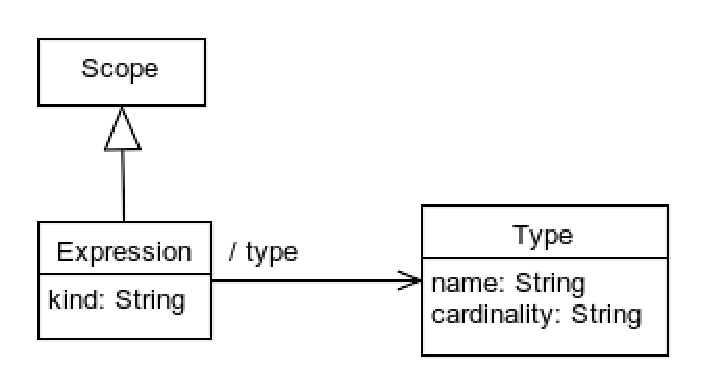
\includegraphics[width=\textwidth]{metamodel/expression}
\caption{Expression Metamodel}
\label{fig:meta:expression}
\end{figure}
